\chapter{Path Planing In Compositional Spaces through Graph Traversals} \label{chap:pathplanning}

\acknowledge{
This chapter is part of work described in Chapter \ref{chap:infeasibilitygliding} and carries the same acknowledgments.
}

A

\begin{figure}[h]
    \centering
    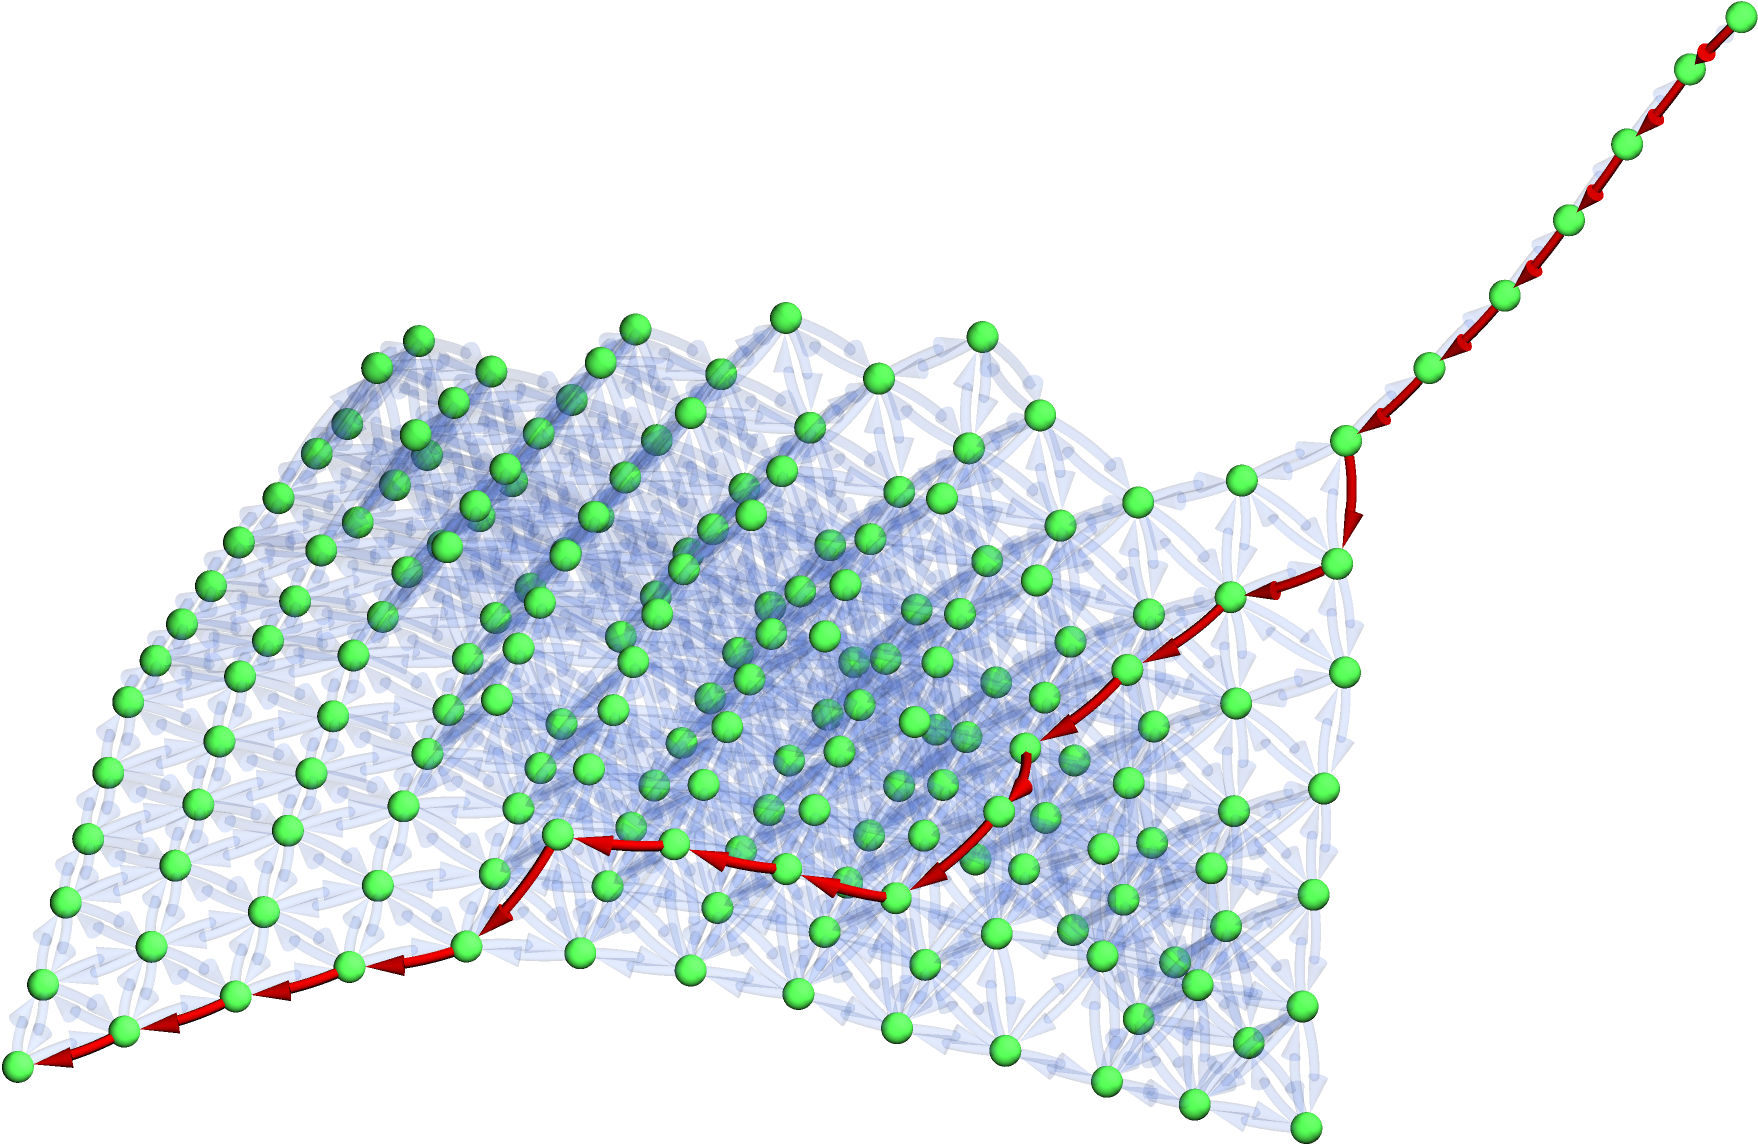
\includegraphics[width=0.9\textwidth]{pathplanning/InfeasibilityGliding_Feasible.png}
    \caption{The subgraph of feasible space extracted from full 3-simplex (tetrahedral) graph in Figure \ref{infeasibilitygliding:fig:glide} constructed by gliding around infeasible region of compositional space. The red path overlaid over directional edges indicates the optimal (least number of transitions) path was identified by the common Dijkstra's algorithm \cite{Dijkstra1959AGraphs}.}
    \label{fig:shortestpath}
\end{figure}

B
\citet{Tandoc2023MiningAlloys}

\begin{figure}[h]
    \centering
    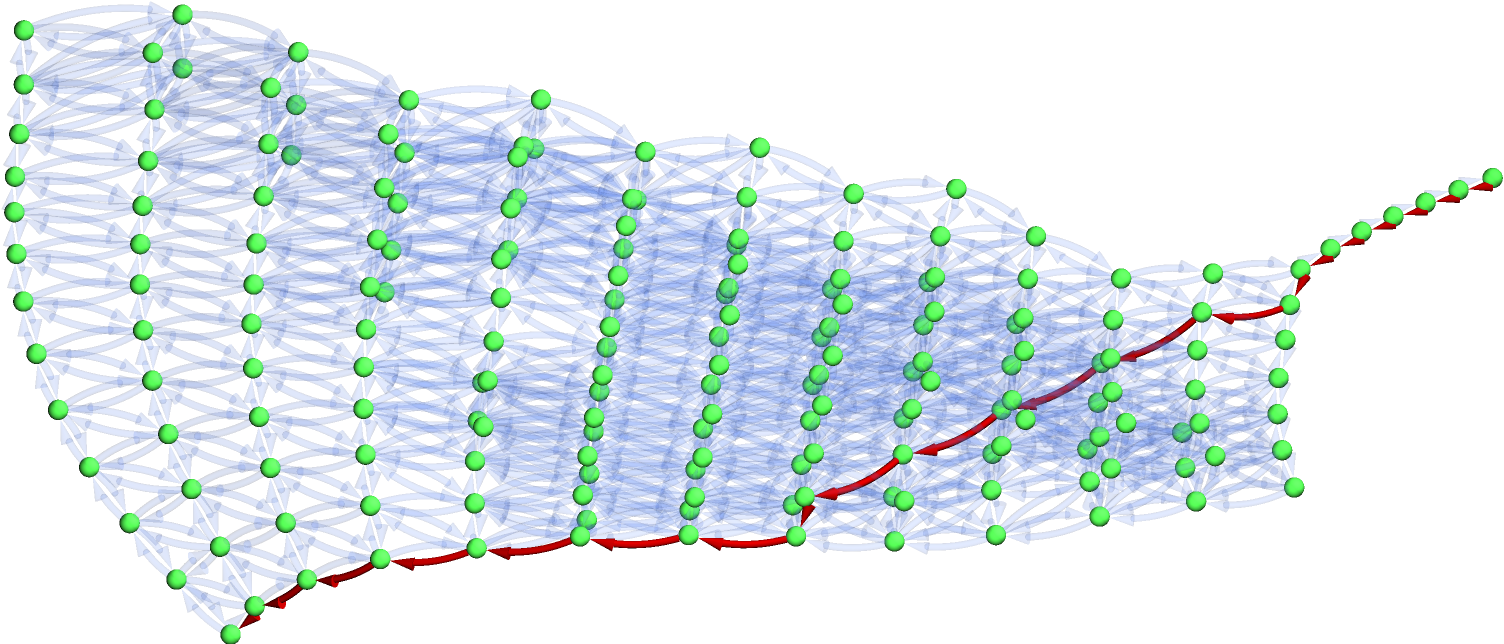
\includegraphics[width=0.9\textwidth]{pathplanning/InfeasibilityGliding_LowGradient.png}
    \caption{The graph from Figure \ref{fig:shortestpath} stretched through distance increases from penalizing high magnitude of gradient in a property value. The graph is approximately relaxed through spring-type energy minimization performed in Wolfram Language. The shortest path is still equally optimal in terms of number of steps but the selection has been biased towards low-gradient region.}
    \label{fig:lowgradient}
\end{figure}

C

\begin{figure}[h]
    \centering
    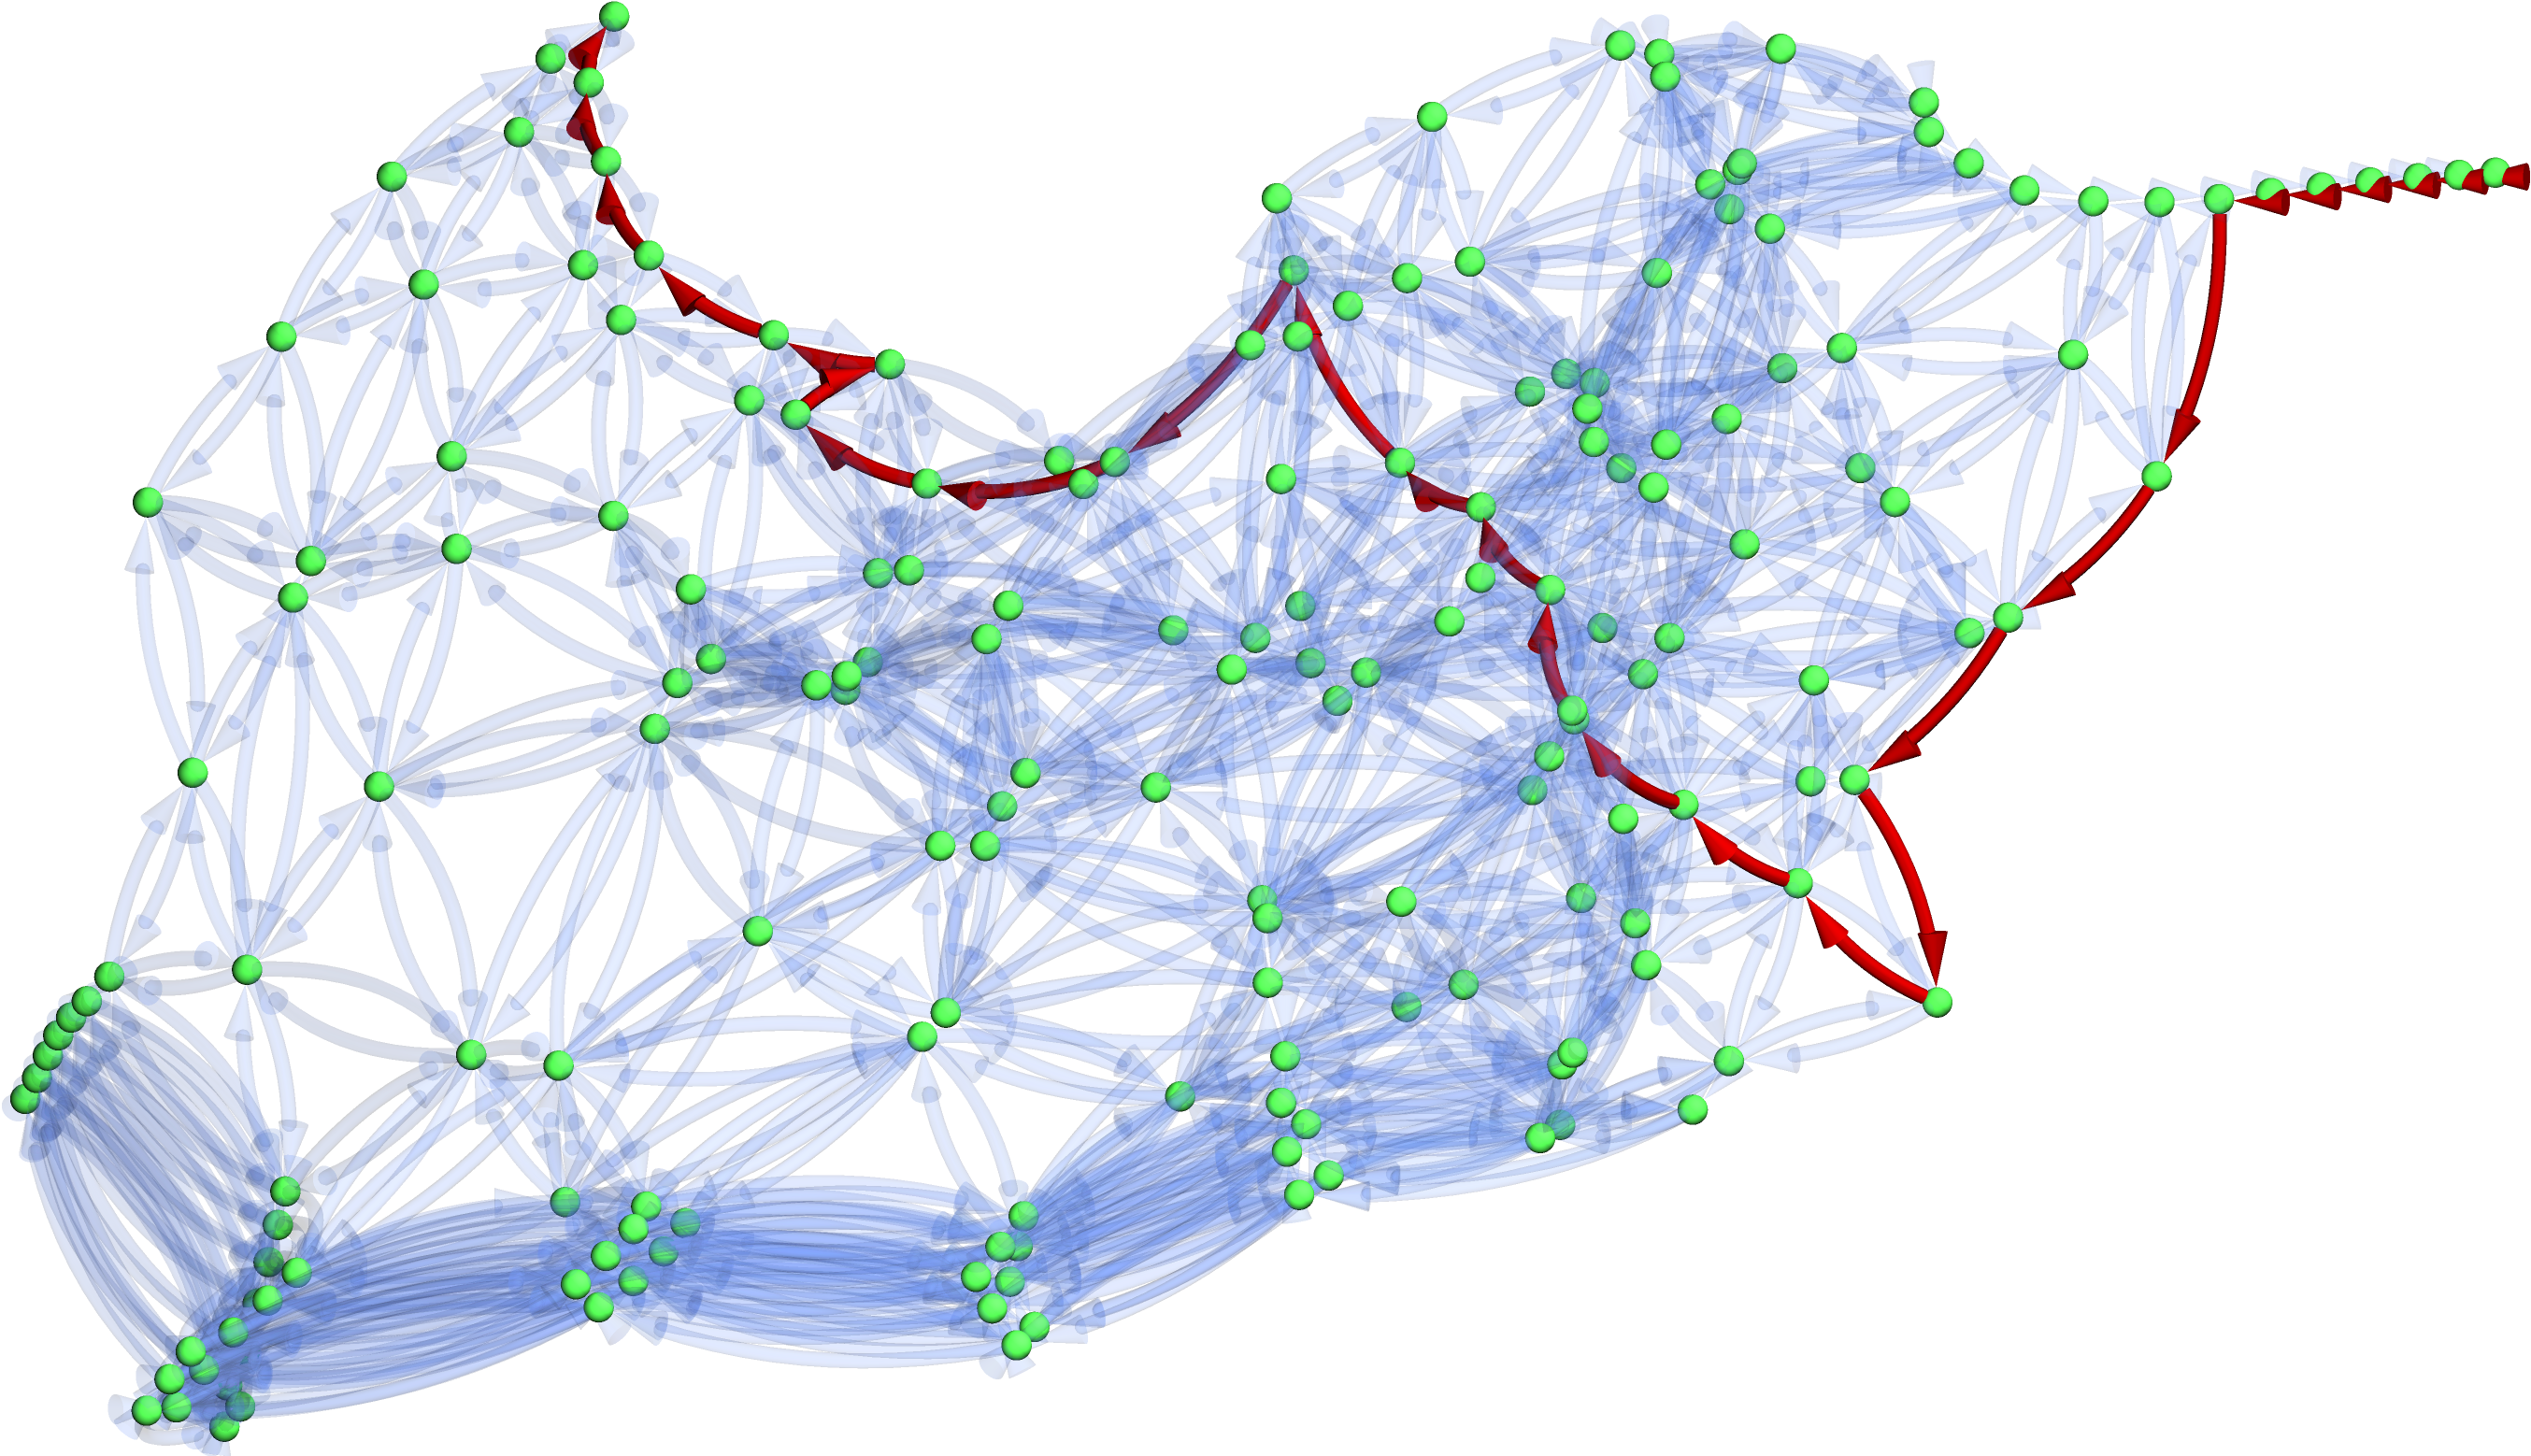
\includegraphics[width=0.9\textwidth]{pathplanning/InfeasibilityGliding_LowGradientSquared.png}
    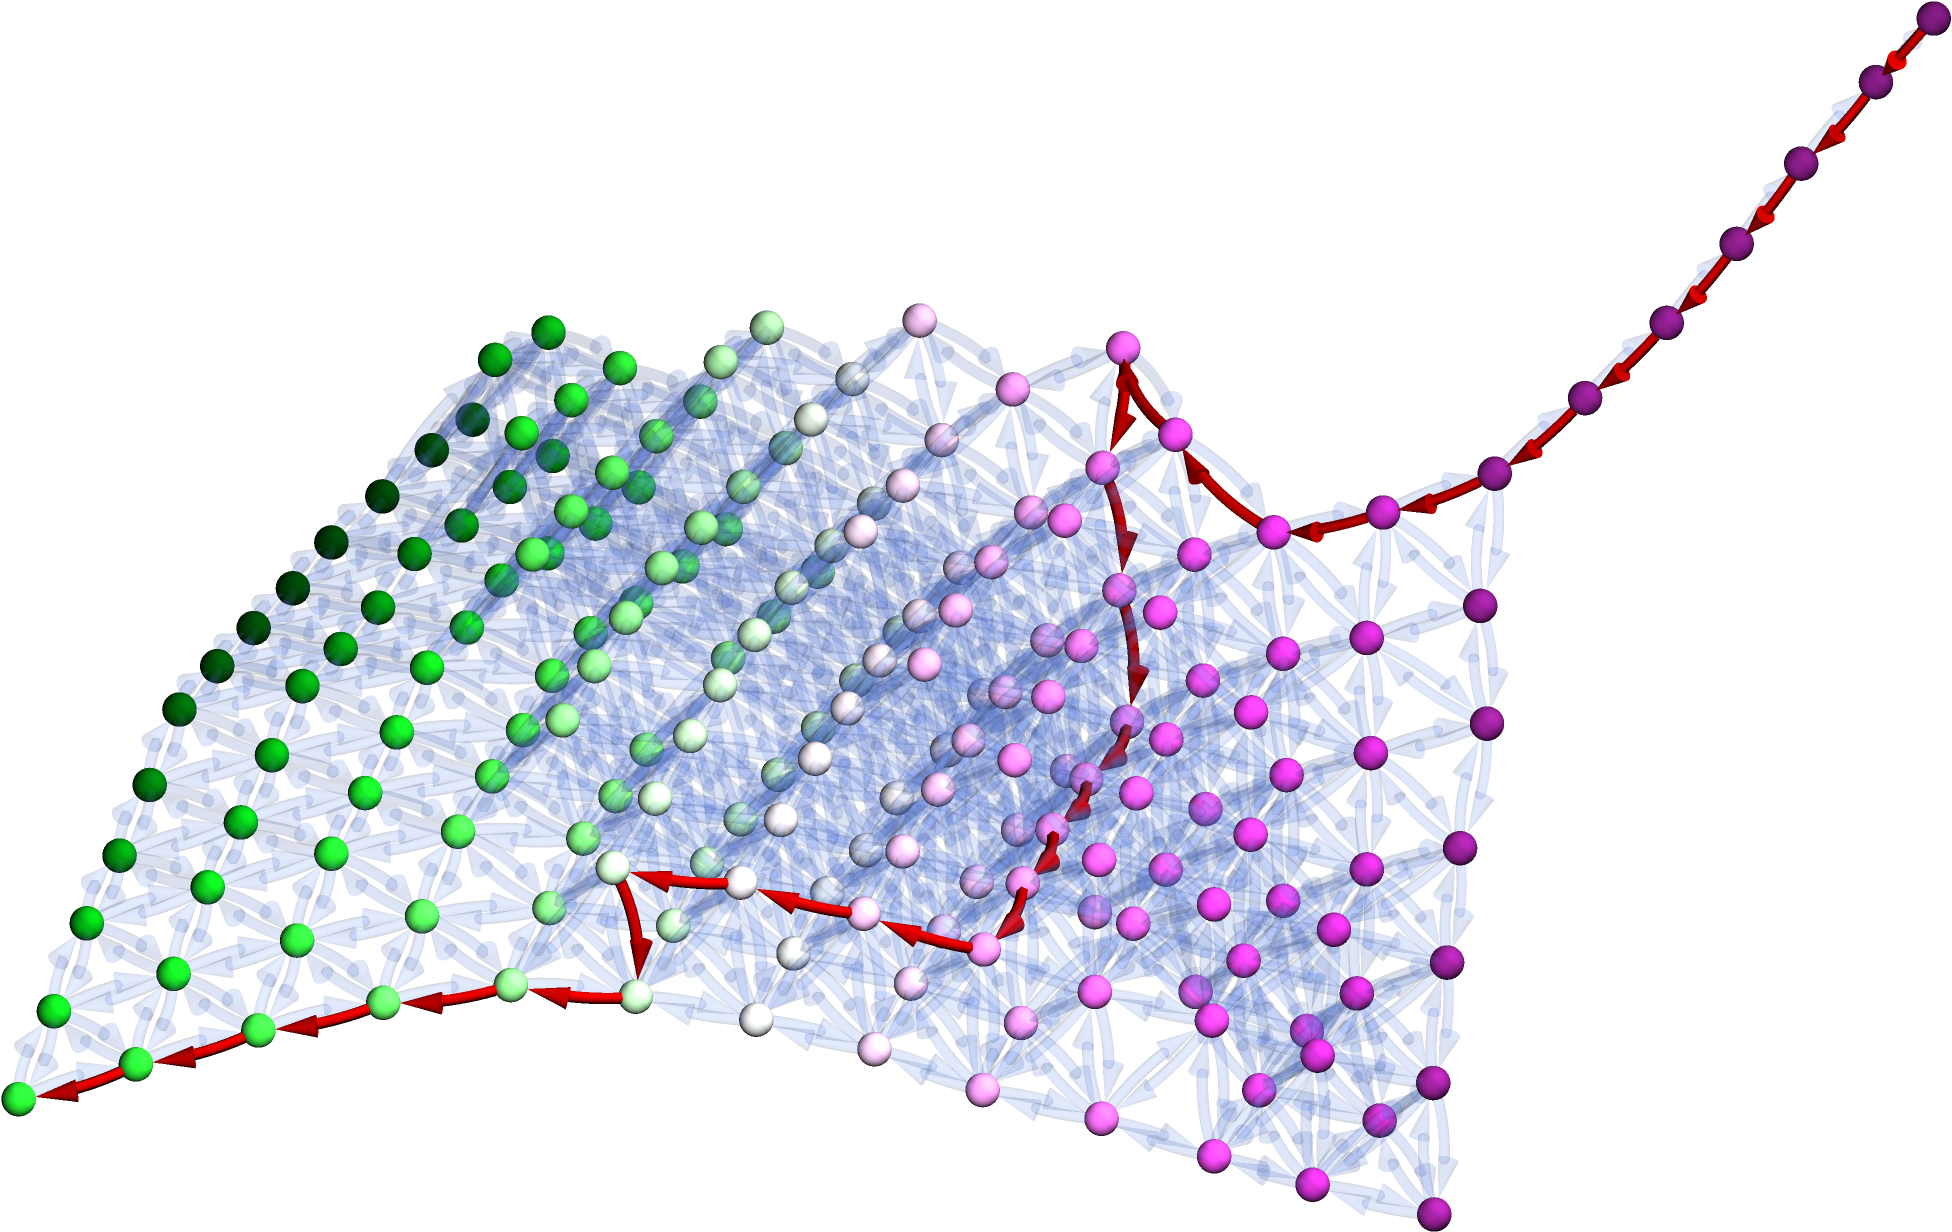
\includegraphics[width=0.9\textwidth]{pathplanning/InfeasibilityGliding_LowGradientSquaredColored.png}
    \caption{Application of a highly non-linear (squared) property gradient magnitude penalty to the inter-node distances causing (top) unrelaxable (local minimum) spatial arrangement of graph nodes, which can be visualized (bottom) through color encoding of property field with path forming "switchbacks" akin to mountain roads that minimize sharp gradients at a cost of 3 additional steps.}
    \label{fig:lowgradientsquared}
\end{figure}

D
Since the transitions between neighboring compositions are described through two unidirectional edges, the distance bias can be used to encode directional properties, such as the property gradient itself. Such method can be used to bias the path into crossing through high property value regions and, similar to those previously described, can be tuned to a desired trade-off with path length.

\begin{figure}[h]
    \centering
    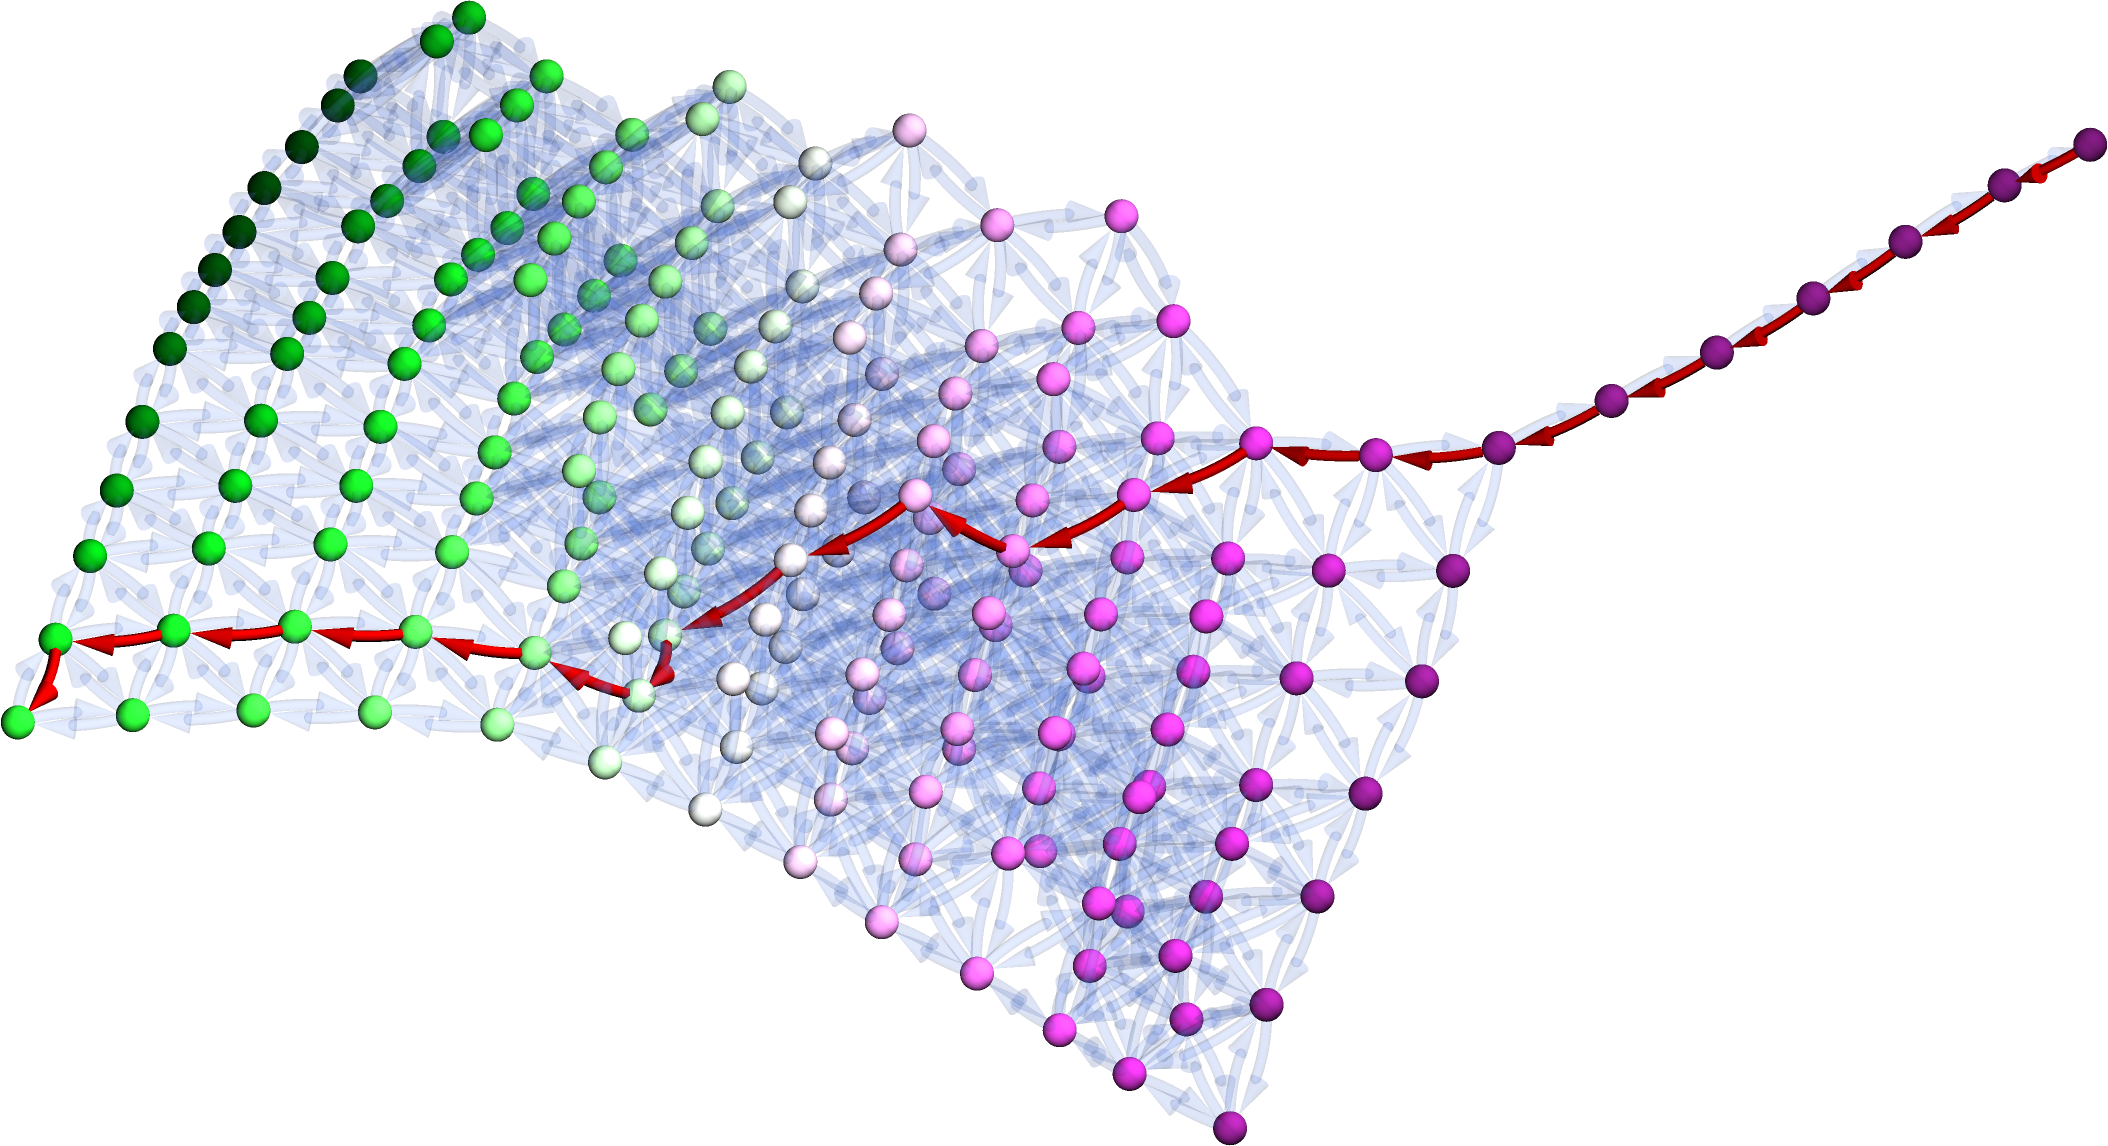
\includegraphics[width=0.9\textwidth]{pathplanning/InfeasibilityGliding_HighRMSAD.png}
    \caption{A selection of an optimal path, similar to one in Figure \ref{fig:shortestpath} but biased towards high property value regions (green) by penalizing going to lower property regions.}
    \label{fig:highrmsad}
\end{figure}



\printbibliography[heading=subbibintoc]